
\chapter{Выборы в Думу}


Сейчас сложно представить, чтобы жители столицы и министры, полицейские и профессура вместе, затаив дыхание, ждали... выборов в Государственную Думу. Ажиотаж, если он и появляется, связан обычно лишь со скандалами и махинациями. Однако в 1905-1906 годах ожидания общества были куда более позитивными.

Документ об изменении положения о выборах, подписанный 11 декабря 1905 года, обозначил новый порядок избирательного процесса. Высочайший указ скорректировал состав землевладельческой и городской курий, позволив увеличить число избирателей, и дал возможность крестьянам усилить своё политическое влияние.
\begin{figure}[h!tb] 
	\centering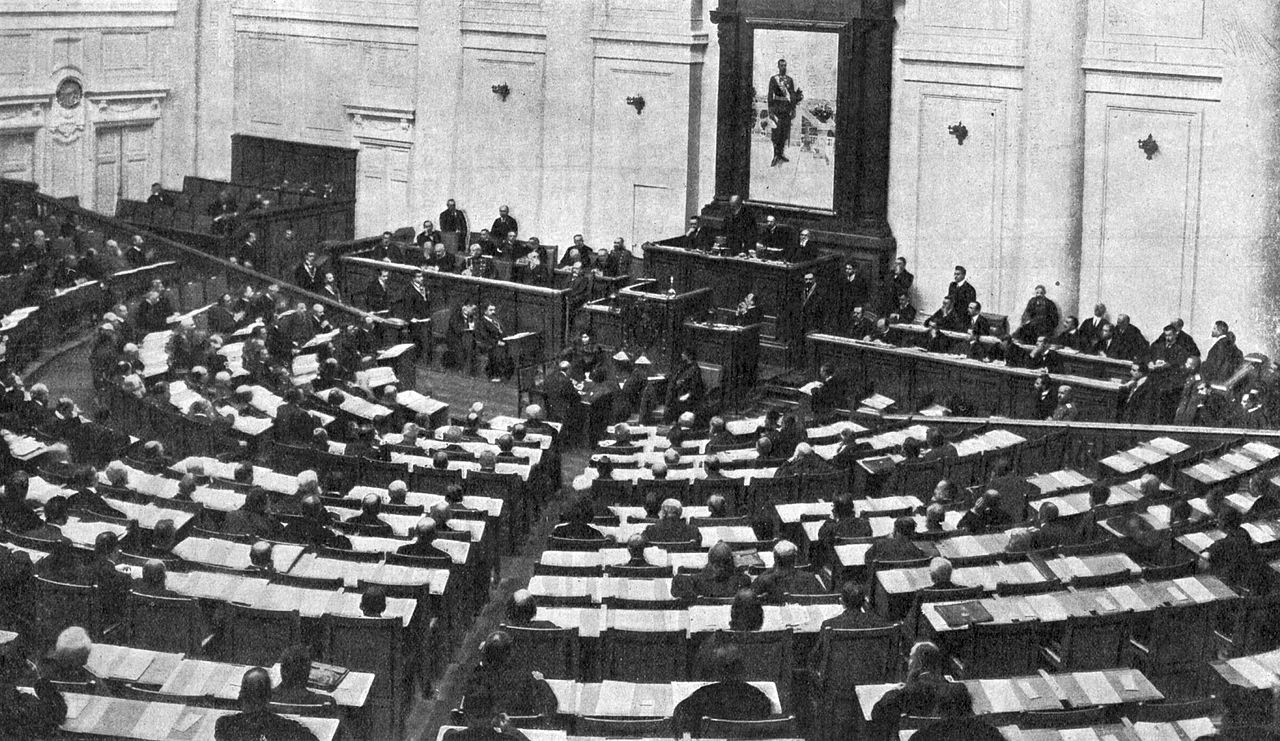
\includegraphics[scale=0.3]{Data/Vybory_V_Dumu/4Sf3k5B8MJ4.jpg}
	%	\label{fig:scipion} % Unique label used for referencing the figure in-text\end{document}
	%	%\addcontentsline{toc}{figure}{Figure \ref{fig:placeholder}} % Uncomment to add the figure to the table of contents%----------------------------------------------------------------------------------------
	\caption{Зал заседаний Государственной Думы }%	CHAPTER 2
\end{figure}

Как раз на крестьянство и делало свою ставку правительство. Да, крестьянину для участия в работе курии нужно было пройти две предварительные стадии, тогда как крупному землевладельцу – ни одной. Однако в итоге именно крестьянская курия собрала около половины голосов. При этом землевладельческая (крупные и мелкие помещики) владела почти четвертью голосов, а городская – чуть больше 1/5.

Конечно, не все были довольны новыми законами. Консервативные круги не желали допускать в Думу радикально настроенное крестьянство и интеллектуалов. Левые и либеральные силы, в свою очередь, были недовольны малым представительством рабочих и отсутствием всеобщего избирательного закона.
\begin{figure}[h!tb] 
	\centering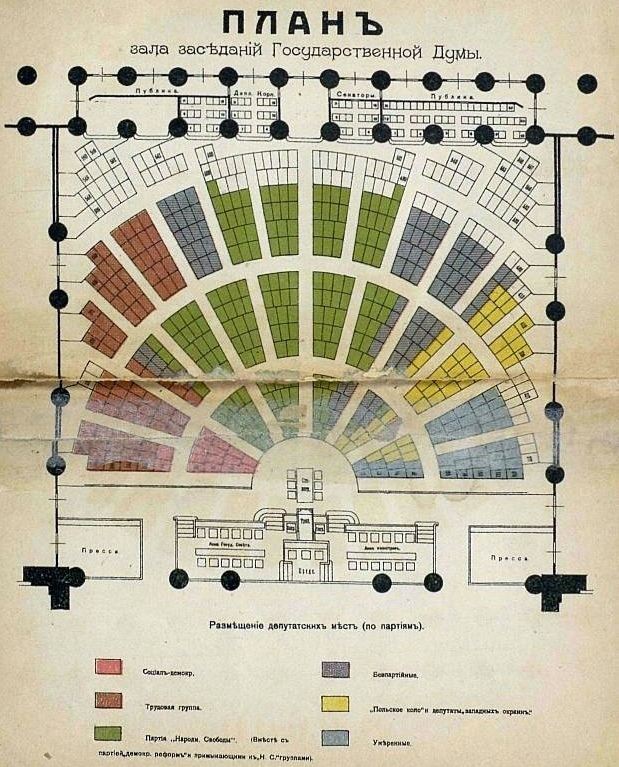
\includegraphics[scale=0.3]{Data/Vybory_V_Dumu/nXeg2HavApM.jpg}
	%	\label{fig:scipion} % Unique label used for referencing the figure in-text\end{document}
	%	%\addcontentsline{toc}{figure}{Figure \ref{fig:placeholder}} % Uncomment to add the figure to the table of contents%----------------------------------------------------------------------------------------
	\caption{План зала}%	CHAPTER 2
\end{figure}

Да, выборы в Думу не были ни всеобщими, ни прямыми, ни равными. В России так и не дали права голоса женщинам, бродягам и студентам, а в деревне голосовали лишь домохозяева. Однако большинство образованной публики воспринимало новый избирательный закон вполне благожелательно. Так, по словам социалиста В.В. Водовозова, от избирательной системы по закону 11 декабря, ко всеобщему избирательному праву оставался один шаг.

При всем при этом, сам ход выборов в I Государственную Думу правительством практически не контролировался. Поэтому в её составе около половины депутатов составили крестьяне, да и рабочие смогли получить неплохое представительство. Увидеть подобную ситуацию в английской палате общин или германском Рейхстаге того времени было просто невозможно.

\begin{figure}[h!tb] 
	\centering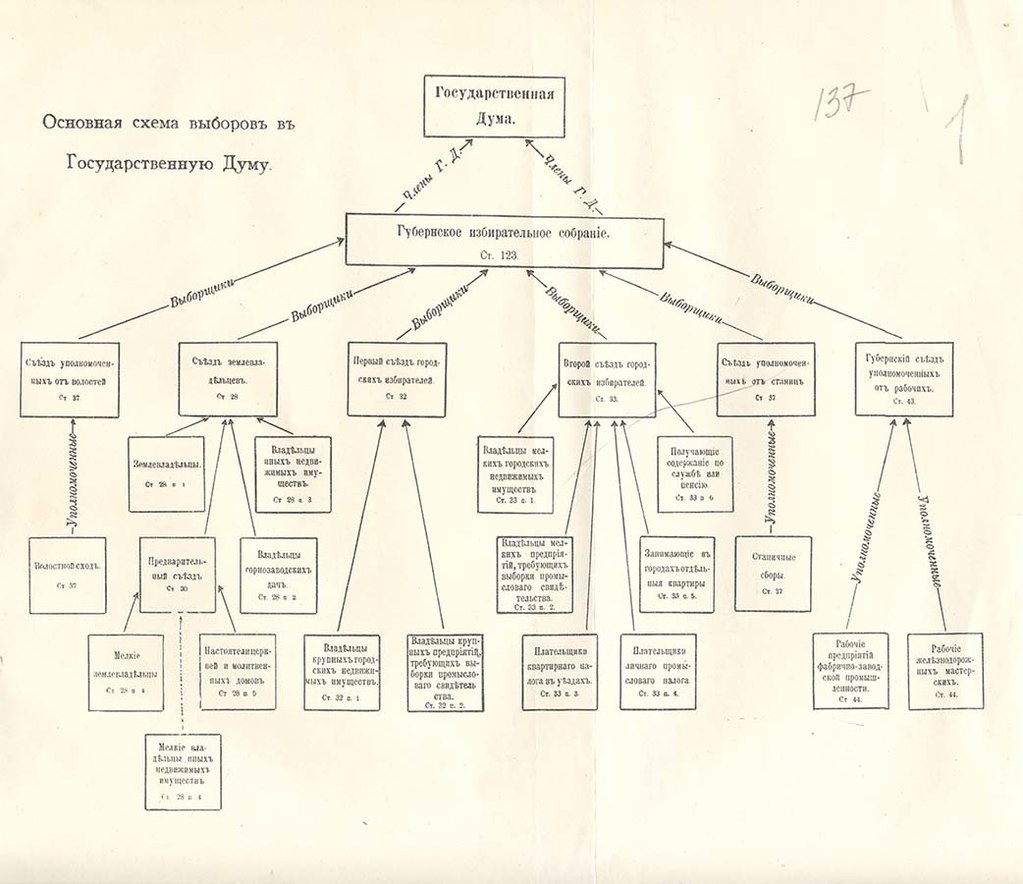
\includegraphics[scale=0.3]{Data/Vybory_V_Dumu/Ho9O9pYTirw.jpg}
	%	\label{fig:scipion} % Unique label used for referencing the figure in-text\end{document}
	%	%\addcontentsline{toc}{figure}{Figure \ref{fig:placeholder}} % Uncomment to add the figure to the table of contents%----------------------------------------------------------------------------------------
	\caption{Схема выборов}%	CHAPTER 2
\end{figure}

Минимальный контроль над выборами объясняется отнюдь не добротой души царя или его министров, а отсутствием эффективных механизмов контроля над новой и незнакомой избирательной системой. Правительство, конечно, активно пользовалось доступными ему средствами влияния на выборы, подключая и местные власти, и правомонархические организации, и Сенат. Многие губернаторы также проявляли недюжинную смекалку в попытках провести "правильных" кандидатов в Думу. Примеры подобного усердия можно найти для каждой из четырех избирательных кампаний.

Например, на выборах в Четвертую Думу нижегородский губернатор А.Н. Хвостов назначил время проведения выборов на 8 утра. Место проведения выборов находилось в восточной части города – Нагорной. Вечером предшествующего выборам дня он повелел развести мосты через Оку и занять все имеющиеся лодки до 10 часов утра соответственно. Когда утром заречная – рабочая – часть Нижнего Новгорода попыталась отправиться на голосование, избиратели обнаружили, что им просто не на чем переправиться через реку.

Однако, несмотря на такие шалости, правительство даже при всем своем желании не могло учесть интересов всех социальных групп, жаждавших представительства в Думе и решения своих собственных проблем. Поэтому выборы в Российской империи часто приводили к парадоксальным союзам: кадеты объединялись со священниками, министерские бюрократы агитировали за оппозицию, а клирики голосовали за октябристов.

Весь этот хаос, нагромождение условностей и кулуарщина могут создать извращенное представление о Думе, как о неработающем органе власти, созданном лишь для удовлетворения сиюминутных потребностей либеральной общественности. Представления о Государственной Думе, как о бесполезной, фиктивной или подконтрольной правительству структуре вполне могут иметь право на жизнь, однако... просто не находят отражения в реальности. Дума в Российской империи, при всех своих недостатках, являлась примером народного представительства и успешно выполняла свои законотворческие функции.

\begin{figure}[h!tb] 
	\centering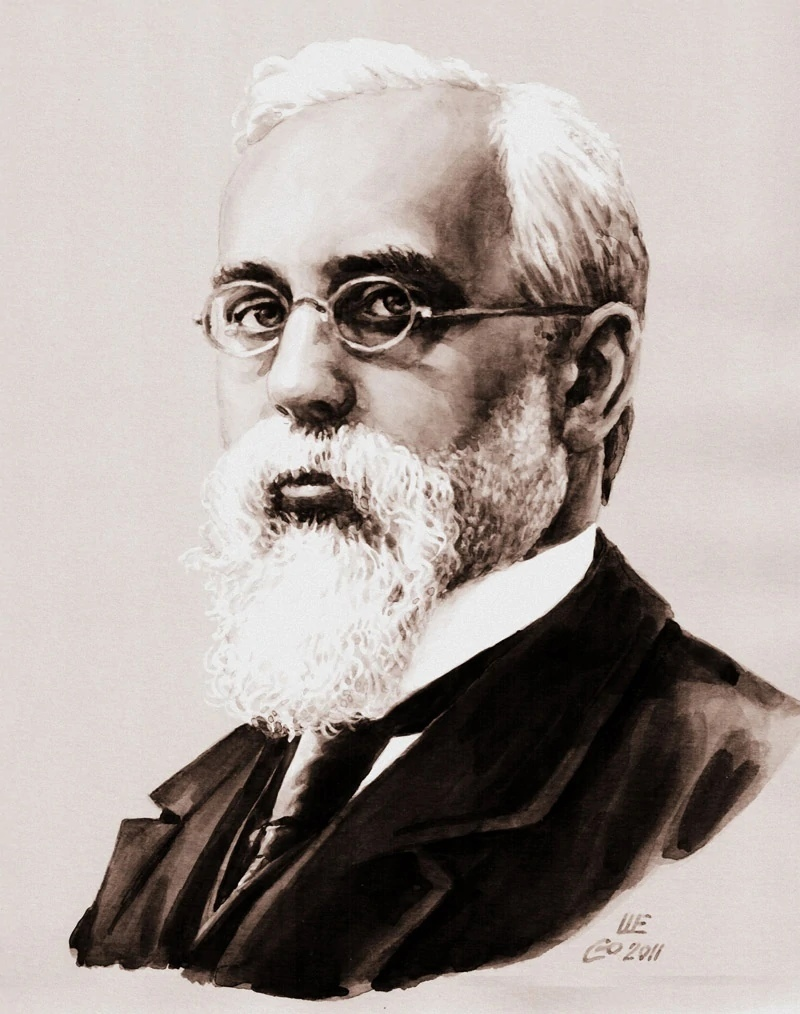
\includegraphics[scale=0.3]{Data/Vybory_V_Dumu/V4ftB5UZj5w.jpg}
	%	\label{fig:scipion} % Unique label used for referencing the figure in-text\end{document}
	%	%\addcontentsline{toc}{figure}{Figure \ref{fig:placeholder}} % Uncomment to add the figure to the table of contents%----------------------------------------------------------------------------------------
	\caption{С.А. Муромцев, председатель I Государственной Думы}%	CHAPTER 2
\end{figure}

Говоря о Первой и Второй Государственных Думах, нужно учитывать, что каждый её элемент, каждая фракция и партия стояли, по сути, в оппозиции правительству. Правые монархисты считали правительство слишком либеральным и были не очень довольны проигрышем на выборах. У националистов, например, польских, поддерживать правительственный курс в принципе не было никакой выгоды. А левые и радикалы вовсе считали Думу фарсом, неспособным решить по-настоящему важные проблемы страны.

К этому прибавляется также и то, что в составе Первой Думы были люди, не умевшие читать и писать, люди, не имевшие опыта законотворческой деятельности (откуда бы ему взяться?), люди, не уверенные в своих политических взглядах, люди, вообще не имевшие политических взглядов, а также персонажи, которые после своего избрания ни разу не посетили Таврический дворец, потому что тратить по 6-10 часов на обсуждение законов – это слишком сложно и утомительно. Знакомо, да?

\begin{figure}[h!tb] 
	\centering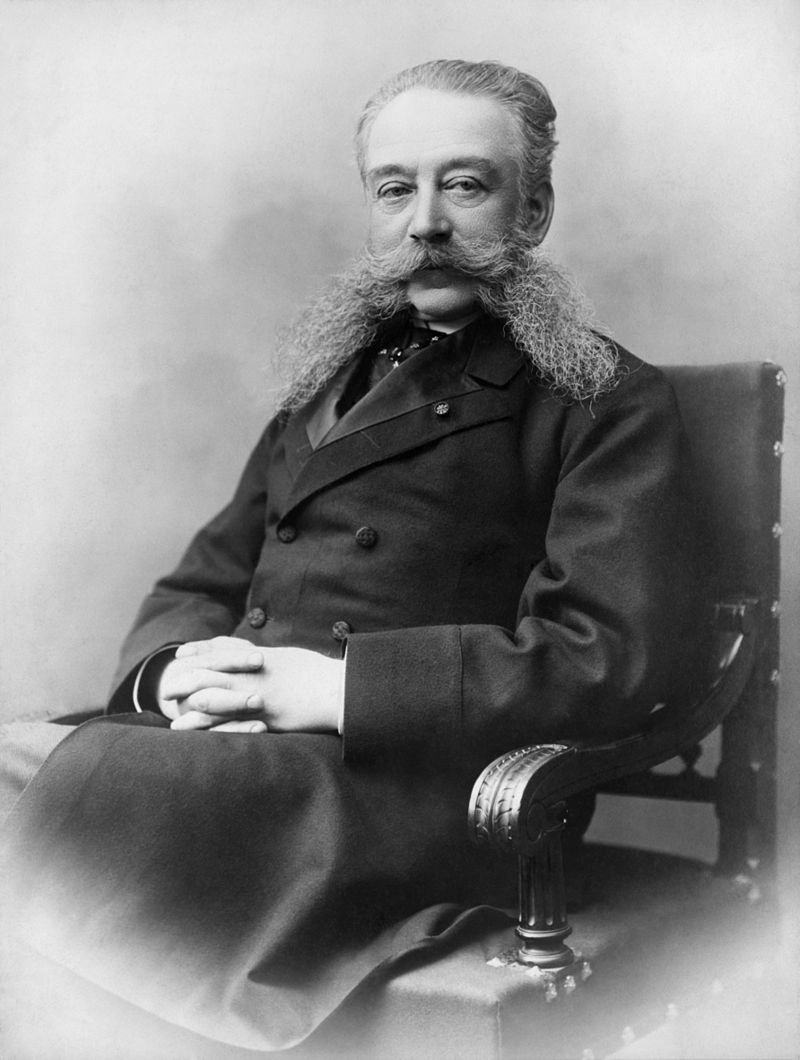
\includegraphics[scale=0.3]{Data/Vybory_V_Dumu/-dKq-zNIERM.jpg}
	%	\label{fig:scipion} % Unique label used for referencing the figure in-text\end{document}
	%	%\addcontentsline{toc}{figure}{Figure \ref{fig:placeholder}} % Uncomment to add the figure to the table of contents%----------------------------------------------------------------------------------------
	\caption{И.Л. Горемыкин, председатель Совета министров 22.04. - 08.07. 1906 г.}%	CHAPTER 2
\end{figure}

Так или иначе, Государственная Дума стала тем самым органом власти, который не позволял более назвать монархию в России "абсолютной". Несмотря на то, что правительство гнуло свою линию в проведении отдельных проектов, именно мнение депутатов было залогом успешного проведения закона. Если правительство или отдельные министры не могли наладить с Думой контакт – их проекты тормозились или вовсе отклонялись. Поэтому председателям и членам Совета министров приходилось аккуратно выстраивать линии взаимодействия с Думой, посещать пленарные заседания, собрания партий, выказывать депутатам свое уважение и продвигать свои проекты не всегда легальными и формальными путями.

Совсем отмахнуться от Думы и её участия тоже не получалось. Утвердить проект без участия Думы было не так просто, как может показаться на первый взгляд. Все инциденты с проведением законов мимо неё можно пересчитать по одному пальцу одной руки. Да и царь-император не злоупотреблял своим правом вето, применив его только два раза.

Самое главное предубеждение против Государственной Думы Российской империи заключается в том, что она не смогла решить те самые масштабные проблемы для чего, казалось бы, и созывалась. Этот факт часто используется для доказательства неэффективности Думы в целом и выстроенной после 1905 года политической системы принятия властных решений.

\begin{figure}[h!tb] 
	\centering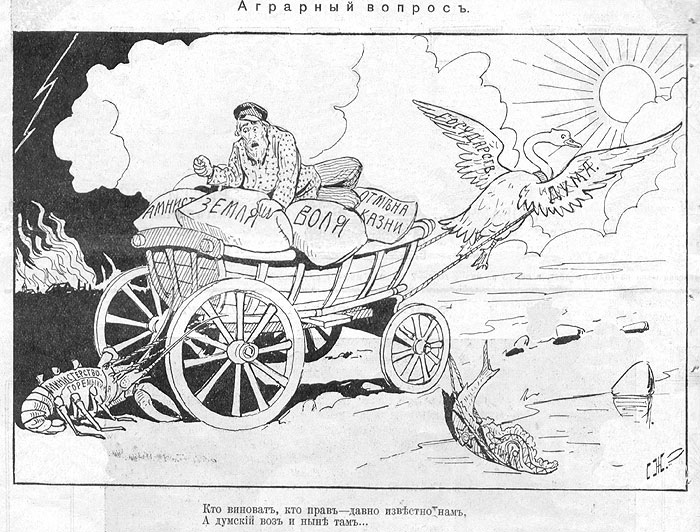
\includegraphics[scale=0.3]{Data/Vybory_V_Dumu/3RTS4AwERjs.jpg}
	%	\label{fig:scipion} % Unique label used for referencing the figure in-text\end{document}
	%	%\addcontentsline{toc}{figure}{Figure \ref{fig:placeholder}} % Uncomment to add the figure to the table of contents%----------------------------------------------------------------------------------------
	\caption{Политическая карикатура по басне И.А. Крылова "Лебедь, рак и щука" ("Искры", 1906)}%	CHAPTER 2
\end{figure}

Да, Дума в конечном итоге не смогла решить основные вопросы, которые волновали общество, да и "законотворческой вермишели", в которой терялась депутатская инициатива, было предостаточно.

Однако в этом заключается ирония. I и II Думы, вмещая в себя представителей самых разных идеологий, не могли решать глобальные вопросы из-за своей пестроты, отсутствия опыта и дезорганизованности. А III и IV Думы – более умеренные, опытные и склонные к сотрудничеству – уже не ставили перед собой задачу, да и не имели возможности, решать проблемы радикальным путем.

Самое главное, что нужно понять, разбираясь в работе первых Дум, так это их разнородность, полярность и вытекающую отсюда неспособность к сотрудничеству с правительством. После Третьеиюньского переворота и установления новой политической системы, Дума перестала быть прибежищем для радикалов, что позволило фракциям идти на контакт с правительством П.А. Столыпина и, по сути, принимать действующие и полезные законы, не отвлекаясь на обсуждение заведомо утопических проектов.

\begin{figure}[h!tb] 
	\centering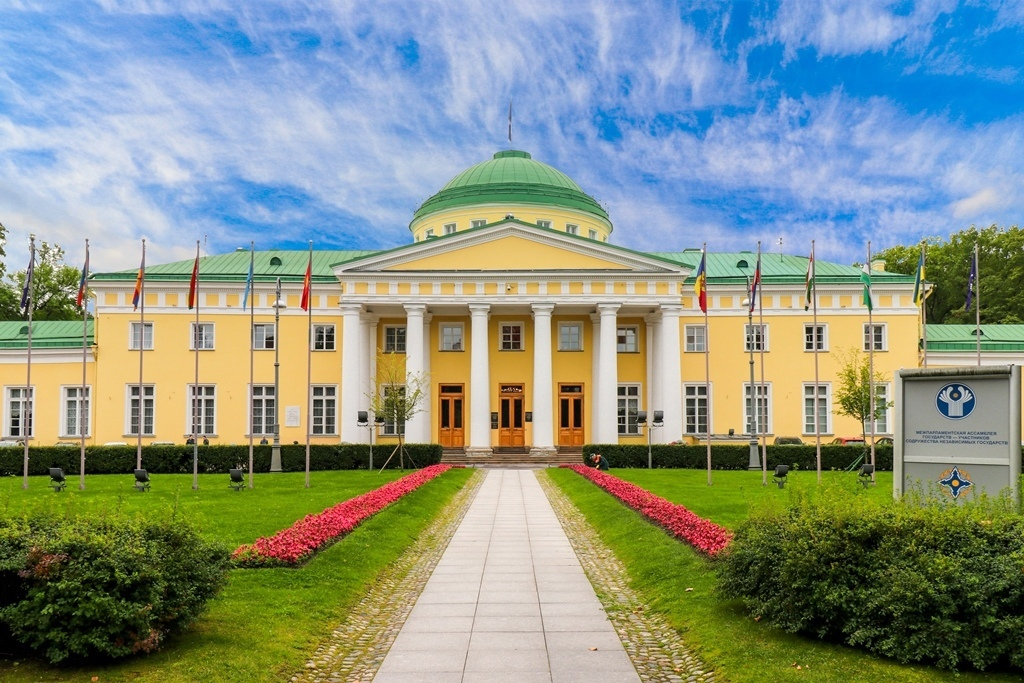
\includegraphics[scale=0.3]{Data/Vybory_V_Dumu/MJ-rW_oCmBM.jpg}
	%	\label{fig:scipion} % Unique label used for referencing the figure in-text\end{document}
	%	%\addcontentsline{toc}{figure}{Figure \ref{fig:placeholder}} % Uncomment to add the figure to the table of contents%----------------------------------------------------------------------------------------
	\caption{здание Таврического дворца}%	CHAPTER 2
\end{figure}


Примером неэффективного использования законотворческой инициативы может служить проект, поданный 33 депутатами-эсерами 6 июня 1906 года, в котором была представлена программа решения аграрного вопроса. Спустя два дня – 8 июня 1906 года, Совет министров принял решение о роспуске Государственной думы в случае продолжения нагнетания обстановки вокруг аграрного вопроса.

Что же вызвало такую реакцию Совета министров и как её трактовать? Прямое давление власти? Угнетение со стороны правительства? Самодержавие пытается вернуть свои позиции? Нет. Всего лишь наивность и радикализм эсеров, которые решили, что выносить на обсуждение такие темы, как национализация природных богатств и отмена частной собственности на землю – это хорошая идея.

Запомните, уважаемые левые депутаты! Если ваши товарищи по цеху отказываются голосовать за ваш проект против всего плохого и за все хорошее – это не значит, что Дума проправительственная, что царь прижал её к ногтю, а все кадеты и октябристы куплены лично Горемыкиным, Столыпиным или Коковцовым.

Это первый текст, по истории Думы в Российской империи. Отпишите, если хотели бы увидеть более подробные заметки о фракционных приколюхах, думском быте, Третьеиюньском перевороте, Госсовете и неформальных связях министров с депутатами.


1. Соловьев К.А. Самодержавие и Конституция: политическая повседневность в России 1906-1917 годах. 2019.
2. Соловьев К.А. Законодательная и исполнительная власть в России.
\\

Автор Илья Агафонов Оригинал \url{https://vk.com/wall-162479647_295278}

\#Агафонов@catx2

\#заметка@catx2
